%%%%%%%%%%%%%%%%%%%%%%%%%%%%%%%%%%%%%%%%%%%%%%%%%%%%%%%%%%%%%%%%%%%%%%%%%%%%%%%%%%%%%%%%%%%%%%%%%%%%%%%%%%%%%%
%%	Licencia:		Este documento se distribuye bajo licencia (CC BY 4.0) Usted puede encontrar un resumen %%
%%					de la licencia en http://creativecommons.org/licenses/by/4.0/deed.es					%%
%%																											%%
%%	-----------------------------------------------------------------------------------------------------	%%
%%																											%%
%%	Plantilla:		exi-examen																				%%
%%	Descripción:	exi-examen.tex es una plantilla para realizar exámenes escritos en formato LaTeX		%%
%%	Autor:			Ing. Alfonso Ramos Michel																%%
%%	Fecha:			9 de diciembre de 2013																	%%
%%	Revisión:		UNO-A																					%%
%%	Paquetes:		inputenc																				%%
%%					babel																					%%
%%					graphicx																				%%
%%					amsmath																					%%
%%					geometry 																				%%
%%					fancyhdr																				%%
%%	Comandos:		\ExiEscuela		Para definir la institución educativa donde se realiza el examen.		%%
%%					\ExiCarrera		Para definir la carrera que se realiza.									%%
%%					\ExiMateria		Para definir la materia que se cursa.									%%
%%					\ExiParcial		Para definir el parcial del cual se realiza el examen.					%%
%%					\informacion	Muesta un recuadro donde poder dar instrucciones al alumno.				%%
%%					\datos			Muestra una línea para el nombre del alumno y la fecha de realización.	%%
%%					\pregunta		Permite introducir (dentro del entorno enummerate) una pregunta o el 	%%
%%									planteamiento de un problema.											%%
%%%%%%%%%%%%%%%%%%%%%%%%%%%%%%%%%%%%%%%%%%%%%%%%%%%%%%%%%%%%%%%%%%%%%%%%%%%%%%%%%%%%%%%%%%%%%%%%%%%%%%%%%%%%%%




\documentclass[letterpaper,11pt]{article}

\usepackage[utf8]{inputenc}
\usepackage[spanish,mexico]{babel}
\usepackage{graphicx}
\usepackage{amsmath}
\usepackage{amsthm}
\usepackage{amsfonts}
%\usepackege{amssymb}
\usepackage[hmargin=1in, vmargin=1in]{geometry}
\usepackage{fancyhdr}
\pagestyle{fancy}


\usepackage{hyperref}
\hypersetup{
    colorlinks=true,
    linkcolor=blue,
    filecolor=magenta,      
    urlcolor=cyan,
}

\urlstyle{same}

\usepackage{tasks}
\lhead{\ExiCarrera}
\chead{\ExiMateria}
\rhead{\ExiParcial}
\cfoot{\ExiEscuela}
\renewcommand{\headrulewidth}{0.4pt}
\renewcommand{\footrulewidth}{0.4pt}

\providecommand{\abs}[1]{\lvert#1\rvert}
\providecommand{\norm}[1]{\lVert#1\rVert}

%=================================================================================
%	Definición de comandos
%=================================================================================
\newcommand{\informacion}[1]{
\begin{center}
\fbox{\fbox{\parbox{\textwidth}{{\footnotesize#1}}}}
\end{center}
\vspace{5mm}}
\newcommand{\datos}{\makebox[0.7\textwidth]{Nombre:~\hrulefill} Fecha:~\hrulefill}
\newcommand{\pregunta}[2]{\item{#2}~{(#1 puntos)}\\ \vspace{5mm}						       
			{\bf Solución}}														  
%	Los siguientes comandos hay que definirlos desde aquí.								    %
\newcommand{\ExiCarrera}{Matemáticas para las Ciencias III.}											  %%%
\newcommand{\ExiMateria}{\textbf{Tarea I}}														%%%%%%%%%%%%%%%%%%%%%%%%%%%%%
\newcommand{\ExiParcial}{Entrega: Miércoles 5 de octubre}														  %%%
\newcommand{\ExiEscuela}{\textbf{Facultad de Ciencias, UNAM}}	                		    %

%=================================================================================
%	Aquí comienza lo bueno, a definir el examen!!!!
%=================================================================================
\begin{document}



%%%%%%%%%%%%%%%%%%%%%            CARÁTULA            %%%%%%%%%%%%%%%%%%%%%%%%%
\setlength{\unitlength}{1cm}
\thispagestyle{empty}
\begin{picture}(18,4)
\put(-0.5,1.2){
\includegraphics[scale=.25]{unam1.png}}
\put(13.5,1){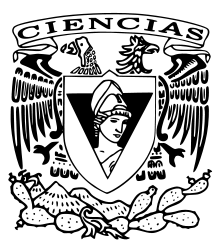
\includegraphics[scale=.35]{fciencias1.png}}
\end{picture}

\begin{center}
\vspace{-134pt}
\textbf{\large Matemáticas para las Ciencias III. }\\[0.2cm]
\textbf{ Semestre 2021-1}\\[0.2cm]
Prof. Pedro Porras Flores\\[0.2cm]
Ayud. Irving Hérnandez Rosas \\ [0.2cm]
%Ayud. Carlos Rodolfo Barrera Anzaldot \\ [0.2cm]
\textbf{Tarea I}
\end{center}
\vspace{-10pt}
\rule{17cm}{0.3mm}
\begin{flushright}
\vspace{-3pt}
\end{flushright}

%%%%%%%%%%%%%%%%%%%%%%%%%%%%%%%%%%%%%%%%%%%%%%%%%%%%%%%%%

%%%%%
%\informacion{\large Profesor: Pedro Porras  Flores \\
%porras@ciencias.unam.mx  \\

%Ayudante: María Guadalupe Gómez Farfán\\ 
 %lupis\_2309@hotmail.com\\
 
% Ayudante: Carlos Rodolfo Barrera Anzaldo\\ 
 %crba@ciencias.unam.mx\\}
%%%%
\noindent \textbf{Instrucciones:} Realice las siguientes ejercicios escribiéndolos  de manera clara, los puede realizar en \LaTeX, en un cuaderno etc, pero debe de subir el archivo en la sesión de classrroom en formato pdf para su revisión.

%\section*{La integral}

\begin{enumerate}

% -----------------------------------------------------
% Problema uno
% -----------------------------------------------------


\section*{Métodos de integración}

\subsection*{Integración por partes (2.5 pts.)}
\item Realice las siguientes integrales:
\begin{tasks}(3)
\task $\displaystyle \int x \sin(x) \, dx$
\task $\displaystyle \int x^2 e^x \, dx$
\task $\displaystyle \int x^2 \sin(x) \, dx$
\task $\displaystyle \int x \ln(x) \, dx$
\task $\displaystyle \int e^{x} \sin(x) \, dx$
%\task $\displaystyle \int \dfrac{\ln(x)}{x} \, dx$
\end{tasks}

\subsection*{Integración por sustitución (2.5 pts.)}
\item  Realice las siguientes integrales:
\begin{tasks}(3)
\task $\displaystyle \int \dfrac{\ln(x)}{x} \, dx$
\task $\displaystyle \int e^x \sin(e^x) \, dx$
\task $\displaystyle \int xe^{-x^2} \, dx$
\task $\displaystyle \int x\sqrt{1- x^2} \, dx$
%\task $\displaystyle \int \tan{(x)} \, dx$
\task $\displaystyle \int \dfrac{1}{x \ln(x)} \, dx$
\end{tasks}

\subsection*{Integración por sustitución trigonométrica (2.5 pts.)}
\item  Realice las siguientes integrales:
\begin{tasks}(3)
\task $\displaystyle \int \sqrt{1 - x^2} \, dx$
\task $\displaystyle \int \sqrt{x^2 - 1} \, dx$
\task $\displaystyle \int \dfrac{\sqrt{1 - x^2}}{x^2} \, dx$
\task $\displaystyle \int  \dfrac{1}{x^2 \sqrt{1 - x^2}} \, dx$
\task $\displaystyle \int  \dfrac{1}{ \sqrt{x^2 - 1}} \, dx$
%\task $\displaystyle \int x\sqrt{1+ x^2} \, dx$
\end{tasks}

\subsection*{Integración por fracciones parciales (2.5 pts.)}
\item  Realice las siguientes integrales:
\begin{tasks}(3)
\task $\displaystyle \int \dfrac{x}{x^2 + 5x + 6} \, dx$
\task $\displaystyle \int \dfrac{x^2 +2}{x(x+2)(x-1)} \, dx$
\task $\displaystyle \int \dfrac{x + 1}{x^2(x-1)^3} \, dx$
\task $\displaystyle \int \dfrac{x^3 - 4x + 3}{x^2(x+1)^2} \, dx$
\task $\displaystyle \int  \dfrac{3x^2 + 1}{(x^2 +1 ) (x^2 + x +1)} \, dx$
%\task $\displaystyle \int \dfrac{3x^2 -1}{(x^2 +1)^2} \, dx$
\end{tasks}

 \end{enumerate}




\end{document}
